\documentclass{beamer}
\usepackage[english]{babel}
\usepackage[utf8]{inputenc}
\usepackage{multicol}
\usepackage{graphicx}
\usepackage{subfig}
%\usepackage[shortlabels]{enumitem}
\usepackage{amsmath,amsthm, amssymb, latexsym}

\usetheme{Frankfurt}
\usefonttheme[onlymath]{serif}
\setbeamertemplate{caption}[numbered]
\setbeamertemplate{enumerate items}[default]
\usepackage[orientation=landscape, size=a0]{beamerposter}

\usepackage[absolute, overlay]{textpos}
\setlength{\TPHorizModule}{\paperwidth}
\setlength{\TPVertModule}{\paperheight}

\title{\huge Boundary Effects in Stochastic Cyclic Competition Models on a Two-Dimensional Lattice}
\author{\Large M. Lazarus Arnau, Shannon Serrao, Uwe C. T{\"a}uber}
\institute{\normalsize Department of Physics (MC 0435) and Center for Soft Matter and Biological Physics\\ Virginia Tech, Blacksburg, Virginia 24061}
\date{July 26, 2018}

\begin{document}
\begin{frame}{}

%Left Col
\begin{textblock}{0.32}(0.01,0.015)
    \begin{block}{Introduction}
        \begin{figure}[h]
            \centering
            \subfloat[]{{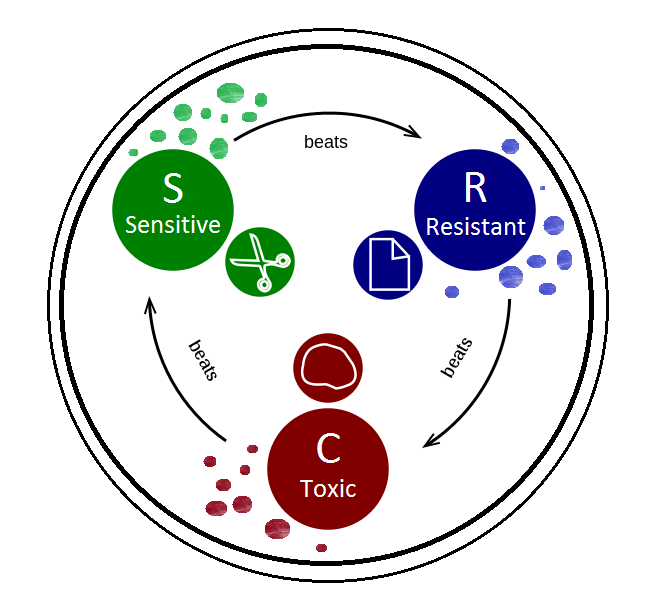
\includegraphics[width=0.4\linewidth]{images/ecolirps.png} }}
            \subfloat[]{{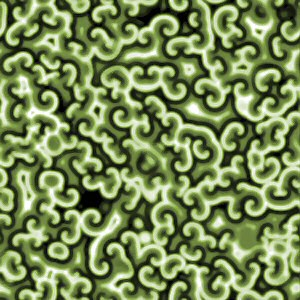
\includegraphics[width=0.4\linewidth]{images/Belousov-Zhabotinsky.jpg} }}
            \caption{(a) Cyclic dominance in \textit{E. -Coli} (b) Spiral pattern formation in the Belousov-Zhabotinsky reaction}
            \label{fig:images}
        \end{figure}
        A number of systems in the fields of ecology, epidemiology, and chemistry
        follow a paradigm of cyclic dominance (e.g. certain subspecies of Lizards in
        California, experiments on cyclically competing \textit{E. -Coli} bacteria, and
        Belousov Zhabotinsky reactions). The formation of noise-induced and -stabilized
        spiral patterns in this class of system is captured by the spatially-extended 
        May-Leonard (ML) model. The formation of these spirals is in stark contrast
        to the species clustering seen in the Rock-Paper-Scissors (RPS).        
    \end{block}
    \begin{block}{The RPS Model}
        The RPS Model is defined by the following binary reactions:
        \begin{itemize}
            \item Replacement Reaction:
            \begin{align*}
                &AB \rightarrow AA\\
                &BC \rightarrow BB\\
                &CA \rightarrow CC\\            
                &\text{with rate } \sigma_r
            \end{align*}
            \item Pair Swap / Diffusion Reaction:
            \begin{align*}
                &XY \rightarrow YX \text{ where } X, Y \in \{A, B, C, \varnothing\}\\
                &\text{with rate } D_r
            \end{align*}
        \end{itemize}
    \end{block}
    \begin{block}{The May-Leonard Model}
        The ML Model is defined by the following binary reactions:
        \begin{itemize}
            \item Predation Reaction:
            \begin{align*}
                &AB \rightarrow A \varnothing \\
                &BC \rightarrow B \varnothing \\
                &CA \rightarrow C \varnothing \\            
                &\text{with rate } \sigma_m
            \end{align*}
            \item Reproduction Reaction:
            \begin{align*}
                &A \varnothing \rightarrow AA\\
                &B \varnothing \rightarrow BB\\
                &C \varnothing \rightarrow CC\\            
                &\text{with rate } \mu
            \end{align*}
            \item Pair Swap / Diffusion Reaction:
            \begin{align*}
                &XY \rightarrow YX \text{ where } X, Y \in \{A, B, C, \varnothing\}\\
                &\text{with rate } D_m
            \end{align*}
        \end{itemize}

        Previous research has shown that the the May-Leonard system has a (quasi-)stable
        reactive fixed point around $(a^*, b^*, c^*) = \frac{\mu}{3\mu + \sigma}(1, 1, 1)$.
    \end{block}
    \begin{block}{Simulation}
        We initialize a lattice of size $L_x \times L_y$ (unless stated otherwise assume
        $(L_x, L_y) = (256, 512)$) with each cell having a probability $p (A) = 
        p (B) = p (C) = {\rho_0}/{3}$ (where $/rho_0$ is the initial net particle
        density) of being initialized to any given species. The lattice is given 
        a toroidal topology (i.e. $x=0 \text{ is equivalent to } x = L_x$ and likewise
        for $y$). The simulation then proceeds according to the following algorithm:
        \begin{enumerate}
            \item A random coordinate $(x, y)$ is selected from a uniform distribution
                and time is advanced by $\delta t = P^{-1}$ (where $P = L_x \times L_y$).
            \item If that lattice point is not empty, then a nearest neighbor is chosen
                at random. If the cell is empty, the simulation returns to step 1.
            \item One of the possible reactions (according to whether the lattice point
                is governed by the ML or RPS model) is selected at random, and excecuted
                if possible. 
        \end{enumerate}
        The simulation is hence run for a predetermined amount of time. 

        \hskip

        In cases where there are both RPS and ML lattice points, all lattice points
        in the range $0 \leq y \leq d_i$ are governed by the RPS model and all 
        remaining lattice points are governed by the ML model.
    \end{block}
\end{textblock}

\begin{textblock}{0.32}(0.34, 0.0125)
    \begin{block}{}
        \maketitle
        \centering

        We study noise-induced and -stabilized spatial patterns in two distinct stochastic 
        population model variants for cyclic competition of three species, namely the 
        Rock-Paper-Scissors (RPS) and the May-Leonard (ML) models. In two dimensions, 
        it is well established that the ML model can display (quasi-)stable spiral 
        structures, in contrast to simple species clustering in the RPS system. Our 
        ultimate goal is to impose control over such competing structures in systems 
        where both RPS and ML reactions are implemented. To this end, we have employed 
        Monte Carlo computer simulations to investigate how changing the microscopic 
        rules in a subsection of a two-dimensional lattice influences the macroscopic 
        behavior in the rest of the lattice. Specifically, we implement the ML reaction scheme 
        on a torus, except on a ring-shaped patch, which is set to follow the cyclic 
        Lotka-Volterra predation rules of the RPS model. There, we observe a marked disruption of 
        the usual spiral patterns in the form of plane waves emanating from the RPS region, 
        up to a characteristic distance that is set by the diffusion rate in the RPS 
        patch. Furthermore, the overall population density drops considerably in the 
        vicinity of the interface between both regions. 

        \hskip

        Research was sponsored by the U.S. Army Research Office and was accomplished 
        under Grant Number W911NF-17-1-0156. 
    \end{block}
    \begin{block}{Normal Pattern formation}
        
    \end{block}
\end{textblock}

%\begin{textblock}{0.32}(0.67,0.015)
%\end{textblock}
\end{frame}
\end{document}
